%\motto{Use the template \emph{chapter.tex} to style the various elements of your chapter content.}
\chapter{Anwendungsgebiete im Finanzbereich}
\label{trends} % Always give a unique label
% use \chaptermark{}
% to alter or adjust the chapter heading in the running head

\chapterauthor{Lola Bankai, Felix Goos}

\abstract{Dieses Kapitel untersucht das Potenzial von Quantencomputing für den Einsatz im Finanzwesen. Im Zentrum stehen drei besonders rechenintensive Anwendungsfelder: Portfoliooptimierung, Monte-Carlo-Simulationen und Risikbeomessung. Anhand aktueller Forschungsergebnisse und Pilotprojekte wird analysiert, wie Quantenalgorithmen klassische Verfahren ergänzen oder perspektivisch ablösen könnten. Dabei werden sowohl Quantum Annealing als auch gate-basierte Algorithmen wie QAOA, VQE und QAE betrachtet. Darüber hinaus beleuchtet das Kapitel die Rolle führender Technologieunternehmen, Finanzinstitute und internationaler Forschungsinitiativen. Abschließend erfolgt eine kritische Bewertung der technologischen Entwicklungen mit Blick auf konkrete Einsatzmöglichkeiten, bestehende Herausforderungen und strategische Implikationen für die Finanzbranche.}


\section{Einleitung}
Das Finanzwesen zählt zu den datenintensiven und rechentechnisch anspruchsvollen Bereichen der modernen Wirtschaft. Täglich werden riesige Datenmengen analysiert, komplexe Modelle berechnet und Entscheidungen unter Unsicherheit getroffen. Klassische Computersysteme stoßen hierbei zunehmend an ihre Leistungsgrenzen, insbesondere wenn es um die Lösung kombinatorischer Optimierungsprobleme, stochastischer Simulationen oder die Verarbeitung hochdimensionaler Datenstrukturen geht. In diesem Kontext rücken Quantencomputer als potenziell transformative Technologie in den Fokus. Da sie auf den Prinzipien der Quantenmechanik wie Superposition, Verschränkung und Interferenz beruhen, ermöglichen Sie damit neue Arten der Informationsverarbeitung, die bei bestimmten Problemklassen eine exponentielle Beschleunigung gegenüber klassischen Verfahren versprechen.

Erste Forschungsarbeiten und Pilotprojekte belegen, dass Quantenalgorithmen insbesondere in der Portfoliooptimierung, in der Bewertung komplexer Finanzinstrumente sowie im Risikomanagement erhebliche Vorteile bringen könnten. Dabei geht es nicht nur um Rechengeschwindigkeit, sondern auch um die Möglichkeit, realistischere Modelle zu verwenden, die bislang aufgrund ihrer Komplexität nicht praktikabel waren. 

Im weiteren Verlauf dieses Kapitels werden zunächst die zentralen Herausforderungen und Chancen des Quantencomputings im Finanzwesen dargestellt. Anschließend werden die drei wichtigsten Anwendungsfelder beleuchtet: Portfoliooptimierung, Optionsbewertung und Risikobemessung. Darauf folgt eine Übersicht über die zugrunde liegenden Technologien und Algorithmen. Zudem werden führende Akteure, bedeutende Unternehmensinitiativen sowie ausgewählte Forschungsprojekte vorgestellt. Den Abschluss bildet eine Bewertung der Entwicklungen und ein Teilfazit mit Blick auf zukünftige Potenziale.

\section{Relevanz und Problemstellung}
Im Finanzwesen wächst der Bedarf an leistungsfähiger und präziser Datenverarbeitung aufgrund immer komplexerer Finanzinstrumente, hochvolatiler Märkte und anspruchsvoller regulatorischer Anforderungen stetig. Herkömmliche Computersysteme geraten dabei zunehmend unter Druck, da ihre Rechenkapazitäten oft nicht mehr mit der exponentiellen Zunahme an Datenvolumina und Modellkomplexität Schritt halten können. Besonders betroffen sind Bereiche wie die Optimierung von Portfolios, die Bewertung derivativer Finanzprodukte und die Durchführung komplexer stochastischer Risikosimulationen, in denen Vereinfachungen unvermeidbar geworden sind. Diese Vereinfachungen können jedoch die Genauigkeit und Aussagekraft der Modelle deutlich verringern (vgl. \cite{egger_quantum_2020}).

Quantencomputer eröffnen hier ein grundsätzlich neuen Lösungsansatz. Durch ihre Fähigkeit, quantenmechanische Prinzipien wie Superposition und Verschränkung für parallele Berechnungen zu nutzen, ermöglichen sie eine signifikante Effizienzsteigerung bei bestimmten Problembereichen im Finanzsektor. Erste Studien und Pilotanwendungen zeigen, dass quantenbasierte Algorithmen insbesondere kombinatorische Optimierungsprobleme und Simulationen stochastischer Prozesse deutlich schneller und genauer durchführen könnten als klassische Methoden (vgl. \cite{orus_quantum_2019, woerner und egger}). Diese Verbesserungen könnten insbesondere dazu beitragen, komplexere und realistischere Modelle einzusetzen und damit bessere Investitionsentscheidungen und Risikomanagementstrategien zu ermöglichen.

Gleichzeitig bringt die Einführung von Quantencomputern neue Risiken und Herausforderungen mit sich. Besonders kritisch ist die potenzielle Bedrohung der klassischen kryptographischen Verfahren, auf denen heutige Finanzsysteme basieren. Das sogenannte „Harvest Now, Decrypt Later“-Risiko beschreibt ein Szenario, bei dem sensible verschlüsselte Finanzdaten bereits heute abgefangen und später mit ausgereiften Quantencomputern entschlüsselt werden könnten (vgl. \cite{mosca_et_al_cybersecurity_2018}). Die derzeit noch unausgereifte Quantentechnologie stellt zudem Unsicherheitsfaktoren hinsichtlich Stabilität, Skalierbarkeit und Anwendungsreife dar.

Daher steht das Finanzwesen aktuell an einer entscheidenden Wegmarke: Die vielversprechenden Chancen des Quantencomputings müssen gegen die neuartigen Risiken abgewogen werden. Eine strategische Auseinadersetzung und praxisnahe Forschung in diesem Technologiefeld sind somit unerlässlich, um die kommenden Veränderungen proaktiv zu gestalten und zugleich bestehende Infrastrukturen effektiv abzusichern (vgl. \cite{egger_quantum_2020, orus_quantum_2019}).


\section{Wichtige Anwendungsfelder (Praxis \& Theorie)}

Die Potenziale von Quantencomputern im Finanzsektor lassen sich beispielhaft an drei spezifischen Anwendungsfeldern aufzeigen. Diese Bereiche zeichnen sich durch hohen Rechenaufwand, komplexe mathematische Modelle und große Praxisrelevanz aus. Im Fokus stehen insbesondere Probleme, die für klassische Computermethoden zunehmend schwer zu bewältigen sind. Quantenbasierte Verfahren könnten hier nicht nur eine erhebliche Effizienzsteigerung bewirken, sondern auch eine qualitative Verbesserung der Ergebnisse ermöglichen.

Im Folgenden werden die drei Anwendungsgebiete gennant und näher untersucht:
Portfoliooptimierung
\begin{itemize}
    \item{\textbf{Portfoliooptimierung}}
\begin{itemize}
        \item{Effiziente Zusammenstellung und laufende Optimierung großer, diversifizierter Portfolios.}
        \item{Potenzial: Schnelle und genauere Bestimmung optimaler Asset-Allokationen mithilfe quantenbasierter Optimierungsverfahren.}
\end{itemize}
\item{\textbf{Optionsbewertung (Monte-Carlo-Methode als Kern)}}
\begin{itemize}
        \item{Komplexe Modellierungen und Bewertung derivativer Finanzinstrumente.}
        \item{Potenzial: Höhere Präzision und Geschwindigkeit in der Berechnung der Optionspreise sowie in der Modellierung relevanter Marktszenarien.}
\end{itemize}
\item{\textbf{Risikomessung und stochastische Simulation (Monte-Carlo-Methode als Kern)}}
\begin{itemize}
        \item{Durchführung umfangreicher Monte-Carlo-Simulationen und präzise Risikomessung bei dynamischen Marktentwicklungen.}
        \item{Potenzial: Deutlich verbesserte Simulationsergebnisse und realistischere Risikoprofile durch quantenunterstützte stochastische Verfahren.}
\end{itemize}
\end{itemize}

Im Folgenden Abschnitt wird kurz ein Exkurs zur Monte Carlo Simulation als Grundlage eingeschoben. Darauf folgt in den weiteren Abschnitte sowohl die theoretischen Grundlagen als auch erste praktische Implementierungen auf aktueller Quantenhardware. Ziel ist es, das Potenzial quantenbasierter Verfahren im Vergleich zu klassischen Methoden realistisch einzuordnen und mögliche technologische Durchbrüche zu identifizieren.



\subsection{Exkurs Grundlage Monte Carlo Simulation - Kern Methode}
Bevor im weiteren genau auf die Optionsbewertung und die Risikomessung und stochastische Simulation eingegangen wird, wird zuerst die Monte Carlo Simulation als Kern Methode behandelt.

Die Bewertung von Anlagen und Portfolios bedingt eine enorme Komplexität durch die unvollkommene Verteilung von Informationen auf Finanzmärkten. Entscheidungen über Risikostrategien, Bewertungen und Investitionen müssen häufig in Situationen getroffen werden, in denen wirtschaftliche Verläufe nicht direkt einsichtig sind. Hierbei greifen Marktteilnehmer auf Schätzungen, Wahrscheinlichkeiten und historische Daten zurück, um zukünftige Entwicklungen zu bewerten. 

 Als zentrales Werkzeug in diesem Bereich kommt die Monte-Carlo-Simulation zum Einsatz. Sie eignet sich besonders zur Schätzung von Lösungen analytisch komplexer oder schwer lösbarer mathematischer Probleme. Dabei werden mithilfe statistischer Verfahren und Zufallsstichproben verschiedene Szenarien eines Systems wiederholt simuliert, um Erwartungswerte oder Wahrscheinlichkeiten näherungsweise zu bestimmen (vgl. \cite{orus_quantum_2019}).

Typische Anwendungsfelder dieses stochastischen Ansatzes sind: Optionsbewertung (Pricing von Derivaten, deren Auszahlung vom zukünftigen Preisverlauf eines Basiswerts abhängt) und Risikobemessung (Berechnung des Value at Risk für ein Portfolio über einen Zeithorizont) (vgl. \cite{orus_quantum_2019}). 

Sowohl die Optionsbewertung als auch die Risikobemessung stellen zentrale Aufgaben im Finanzwesen dar, bei denen zukünftige, stochastisch unsichere Größen quantifiziert werden müssen. Aufgrund der Komplexität moderner Finanzinstrumente und der hohen Dimensionalität der zugrunde liegenden Zufallsprozesse sind analytische Lösungen häufig nicht verfügbar. Die Monte-Carlo-Simulation dient in beiden Anwendungsfeldern als methodisches Fundament, um durch zufällige Stichproben komplexe Erwartungswerte oder Verteilungsquantile numerisch zu vergleichen. Damit bildet sie die Grundlage zahlreicher Bewertungs- und Risikomodelle in Praxis und Forschung.

\subsection{Optionsbewertung}
Die Bewertung von Optionen erfordert häufig numerische Verfahren, da für viele Ausgestaltungen keine geschlossenen analytischen Lösungen existieren. Besonders bei komplexeren Derivaten wie asiatischen Optionen, Barrier-Optionen oder Portfolios von Optionen muss meist numerisch simuliert werden. Optionen stellen Finanzderivate dar, wobei ein Derivat ein Instrument ist, dessen Preisentwicklung von der Entwicklung einer oder mehrerer Anlagen abhängt. Das Monte-Carlo-Verfahren nutzt hierbei eine große Menge an Zufallspfad-Simulationen generiert für die relevanten Prozesse und errechnet aus den Auszahlungen oder Verlusten statistische Kennzahlen. Faktisch wird versucht, den „fairen“ Preis einer Option zu ermitteln. Dazu werden mögliche Pfade, die der Aktienkurs einnehmen könnte, bis zur Fälligkeit simuliert, für jeden Pfad die Auszahlung berechnet und gemittelt (vgl. \cite{orus_quantum_2019}).
 
Damit die Verteilungsmerkmale in der geforderten Genauigkeit erfasst werden können, müssen ausreichend Pfade generiert werden. Das Gesetz der großen Zahlen bestimmt hierbei dass die Schätzung des Erwartungswertes mit der Anzahl N der simulierten Pfade ungefähr mit $1/\sqrt{N}$ konvergiert. Diese Konvergenz ist verhältnismäßig gering. Um die Genauigkeit, um genau eine Einheit zu verbessern, muss die Zahl der Simulationsläufe um das Vierfache erhöht werden. Dadurch steigt die Zahl der Pfade schnell auf eine Millionen oder Milliarden Höhe an.
In der Praxis ist genau das eins der größten Probleme. Komplexe Berechnungen von zum Beispiel Kreditrisiko-Simulationen von Hunderten von Banken und Unternehmen können Tage dauern. Trotz der stetigen Parallelisierung stoßen herkömmliche Methoden aufgrund der Rechenzeit und Kosten an Ihre Grenzen (vgl. \cite{orus_quantum_2019}).

\subsubsection*{Quantenbasierte Methoden zur Optionsbewertung}

Durch methodische Erweiterungen, wie der Quantum Amplitude Estimation (QAE) können Prozesse der klassischen Monte-Carlo Simulation beschleunigt werden. Bei dem Fall der Optionsbewertung, müssen Wahrscheinlichkeitsverteilungen über zukünftige Assetpreise quantenmechanisch kodiert werden. Diesbezüglich wird QAE angewendet, um effiziente Schätzungen des Erwartungswertes, also die Bestimmung des “fairen” Optionspreises, zu gewährleisten. Im Vergleich zur klassischen Monte-Carlo-Methode, die für eine Zielgenauigkeit von $\varepsilon$ etwa $O(1/\varepsilon^2)$ Stichproben benötigt, minimiert QAE diesen Aufwand auf $O(1/\varepsilon)$. Praktisch bedeutet das, dass statt einer Million klassischer Proben rund 1000 Quantenproben ausreichen bei gleichbleibender Akkuratesse (vgl. \cite{lomonaco_quantum_2002, montanaro_quantum_2015}).

In ersten Bewertungs-Workflows wurde dieser theoretische Ansatz bereits auf realer Quantenhardware getestet und demonstriert. Es wurden verschieden Optionsarten mithilfe passender Quantenschaltungen modelliert und darauf folgend mit Maximum-Likelihood-Amplitude-Estimation (MLAE) bewertet. Dieses Verfahren ist vorteilhafter als das klassische QAE, da es durch eine flachere Schaltung besser für die NISQ-Geräte geeignet ist. NISQ-Geräte (Noisy Intermediate-Scale Quantum) sind gegenwärtige Quantencomputer mit einer begrenzten Anzahl von Qubits und ohne vollständige Fehlerkorrektur, die bereits erste praktische Anwendungen ermöglichen, jedoch noch anfällig für Störungen und Skalierungsprobleme sind (vgl. \cite{stamatopoulos_option_2020}).

Fehler können durch Kalibrierung von Zwei-Qubit-Gattern gedämpft werden, wodurch bereits aus Drei-Qubit-Schaltungen valide Optionspreise extrahiert werden konnten. Zentrale praktische Hindernisse bleiben jedoch bestehen. Besonders das effiziente Laden von Datenquellen und klassischen Wahrscheinlichkeitsverteilungen auf Quantenhardware stellt sich als kompliziert heraus. Um diese Marktszenarien, wie Asset-Preise, auf Quantencomputern zu verarbeiten, müssen die Daten in einen entsprechenden Quantenzustand überführt werden. Hiefür benötigen die klassischen Verfahren einen exponentiell steigenden Ressourcenaufwand von $O(2^n)$. Eine Lösung bietet Quantum Generative Adversial Networks (qGans), die aus den klassischen Marktdaten die passenden Wahrscheinlichkeitsverteilungen erlernt und anschließend als polynomieller Komplexität als Quantenzustand bereitstellt (vgl. \cite{zoufal_quantum_2019}).

Zusammenfassend wird deutlich, dass QAE in Kombination mit verfahren wie MLAE, iterativen QAE oder variationalen Ansätzen zu einer Beschleunigung klassischer Monte-Carlo-Simulationen führt. In Verbindung mit effizienten Datenlagern wie qGANs rückt der Einsatz solcher Verfahren auf realer Quantenhardware in greifbare Nähe.

\subsection{Risikobemessung und Value at Risk}

Eine der zentralen Herausforderungen im modernen Finanzwesen ist die Risikobemessung. Um drohende Verluste rechtzeitig zu erkennen und gezielt Gegenmaßnahmen zu ergreifen, sind Banken, Investoren und andere Marktteilnehmer in einem hoch volatilen Marktumfeld darauf angewiesen, Risiken genau zu quantifizieren und zuverlässig einschätzen zu können.

Auch in der Risikobemessung stellt die Monte-Carlo-Simulation ein zentrales Instrument dar, insbesondere zur Schätzung von Risikokennzahlen wie dem Value at Risk (VaR) oder dem Conditional Value at Risk (CVaR), die auf der Analyse stochastischer Verlustverteilungen basieren. Der VaR ist ein anerkanntes und gängiges Instrument zur Quantifizierung von Risiko und zeigt den maximalen Verlust an, den ein Portfolio oder eine einzelne Anlageposition innerhalb eines bestimmten Zeitraums und mit einer festgelegten Vertrauens-Wahrscheinlichkeit (in der Regel 95\,\% oder 99\,\%) nicht überschreiten wird (vgl. \cite{springer2025, plos2024}). 
Für Finanzinstitutionen ist der VaR nicht nur methodisch relevant, sondern auch regulatorisch von hoher Bedeutung. Finanzinstitute wie Banken, Versicherungen und Investmentfonds sind gesetzlich verpflichtet, Marktrisiken und Kreditrisiken regelmäßig zu quantifizieren, um ausreichende Kapitalpuffer zu erzeugen. Die Risikokennzahlen dienen darüber hinaus intern der Begrenzung von Handelspositionen, etwa durch tägliche VaR-Limits für einzelne Portfolios oder Trader. Auch in der langfristigen Risikosteuerung, etwa bei Pensionskassen oder Versicherungen, sind VaR und CVaR zentrale Steuerungsgrößen, um sicherzustellen, dass finanzielle Verpflichtungen auch unter Stressszenarien eingehalten werden können (vgl. \cite{orus_quantum_2019}).
Trotz seiner weiten Verbreitung ist der VaR nicht frei von Kritik. Insbesondere die fehlende Subadditivität kann bei der Aggregation von Risiken zu fehlerhaften Einschätzungen führen. Der CVaR wurde als kohärentes Risikomaß eingeführt, um auch die Schwere der Verluste im Extrembereich zu erfassen und gilt in vielen Anwendungen als präzisere Alternative (vgl. \cite{orus_quantum_2019}). 

In der Praxis lassen sich VaR und CVaR nur in einfachen Fällen analytisch berechnen. Komplexe Portfolios mit nicht-normalverteilten Erträgen oder Derivatebestandteilen erfordern numerische Verfahren. Die Monte-Carlo-Simulation ist hier besonders geeignet, um aus vielen simulierten Szenarien empirische Verlustverteilungen abzuleiten und daraus die relevanten Quantile zu bestimmen (vgl. \cite{zoufal_quantum_2019}).

Die Monte-Carlo-Simulation gilt zwar als Standardverfahren zur Schätzung komplexer Verlustverteilungen, stößt jedoch bei steigender Modellkomplexität schnell an ihre Grenzen. Mit zunehmender Anzahl an Risikofaktoren, Anlageklassen oder eingebetteten Derivaten steigt der Rechenaufwand drastisch an. Insbesondere die Ermittlung von Extremrisiken wie dem 99{,}9\,\%\,VaR erfordert Millionen von Simulationsläufen, was selbst auf leistungsstarken Rechnern mit erheblichen Laufzeiten verbunden ist. Für verschachtelte Portfolios kommt es häufig zu sogenannten Nested-Monte-Carlo-Strukturen, bei denen für jedes Szenario zusätzliche Bewertungen durchgeführt werden müssen. Die resultierende Rechenzeit verhindert eine laufende Risikobewertung in kurzen Intervallen und erschwert eine schnelle Reaktion in volatilen Marktphasen (vgl. \cite{bouland_prospects_2020, orus_quantum_2019})


\subsubsection*{Quantenbasierte Methoden zur Risikobemessung und Value at Risk}

In Anbetracht der rechentechnischen Hürden klassischer Risikosimulationen rückt erneut Quantum Computing als vielversprechender Lösungsansatz zunehmend in den Fokus. Besonders relevant ist auch hierbei der Quantum-Amplitude-Estimation-Algorithmus (QAE), der bei der Berechnung stochastischer Erwartungswerte eine quadratische Beschleunigung gegenüber klassischen Monte-Carlo-Verfahren ermöglicht (vgl. \cite{quantumjournal2020, rebentrost_quantum_2018}). Der Vorteil des QAE ist der selbe wie in der Optionsbewertung und lässt sich durch eine Minimierung der Simulationsläufe identifizieren, wodurch eine Zielgenauigkeit $\varepsilon$ erreicht wird, da die Komplexität von $O(1/\varepsilon^2)$ auf $O(1/\varepsilon)$ reduziert wird (vgl. \cite{martin2022}). Dies ist besonders relevant bei der Schätzung seltener Ereignisse wie dem 99{,}9\,\%-VaR, bei dem klassisch Millionen bis Milliarden Pfade erforderlich wären.

Zur Anwendung von QAE im Risikokontext wird ein Orakel-Operator entworfen, der für ein bestimmtes Verlustniveau $x$ anzeigt, ob der simulierte Portfolioverlust dieses Niveau überschreitet. Mittels QAE lässt sich dann die Wahrscheinlichkeit $P(\text{Verlust} > x)$ effizient bestimmen. Durch Variation von $x$ kann so derjenige Schwellenwert ermittelt werden, für den die Überschreitungswahrscheinlichkeit einem definierten Konfidenzniveau entspricht, was exakt der Definition des Value at Risk entspricht. Analog dazu lässt sich auch der Conditional Value at Risk berechnen, indem ein modifizierter Schaltkreis verwendet wird, der den durchschnittlichen Verlust im Überschreitungsfall quantifiziert (vgl. \cite{orus_quantum_2019, egger_quantum_2020}).

Die Umsetzung dieser quantenmechanischen Verfahren erfordert jedoch eine geeignete Repräsentation der Verlustverteilung auf dem Quantencomputer. Dazu müssen komplexe stochastische Prozesse, wie sie etwa durch Marktrisiken und Korrelationen zwischen verschiedenen Risikofaktoren entstehen, in einem Quantenzustand abgebildet werden. Eine direkte Kodierung solcher Verteilungen auf Quantenhardware ist jedoch exponentiell aufwendig, weshalb quantum-native Methoden wie Quantum Generative Adversarial Networks (qGANs) eingesetzt werden. Diese Netzwerke sind in der Lage, aus realen Marktdaten eine Zielverteilung zu lernen und diese in polynomieller Komplexität als Quantenzustand bereitzustellen (vgl. \cite{zoufal_quantum_2019}). Kombiniert mit vereinfachten QAE-Varianten wie dem Maximum-Likelihood-Amplitude-Estimation (MLAE), die flachere Quantenschaltkreise erzeugen, können solche Verfahren auch auf heutiger NISQ-Hardware eingesetzt werden (vgl. \cite{stamatopoulos_option_2020}).

Erste Proof-of-Concept-Studien zeigen, dass quantenbasierte Risikomessung prinzipiell umsetzbar ist. In einer wegweisenden Arbeit demonstrierten Woerner und Egger die Berechnung des VaR für ein vereinfachtes Anleiheportfolio mit Hilfe eines IBM-Q-Prozessors. Trotz der Beschränkung auf wenige Qubits konnten valide Resultate erzeugt werden, die die klassische Berechnung reproduzierten (vgl. \cite{egger_quantum_2020}). Aufbauend darauf wurden in weiteren Studien der potenzielle Ressourcenbedarf für realistische Risikoszenarien analysiert. Diese Arbeiten kommen zu dem Ergebnis, dass für große Portfolios mit vielen Risikofaktoren und hohen Konfidenzniveaus fehlerkorrigierte Quantencomputer mit deutlich größerer Qubit-Anzahl erforderlich wären. Gleichzeitig wurden aber auch Ansätze zur Reduktion der Komplexität untersucht, etwa durch grobe Vorabschätzungen mittels klassischer Simulation oder durch analytische Näherungen innerhalb des quantenbasierten Modells (vgl. \cite{martin2022}).

Auch in der Finanzindustrie wächst das Interesse an quantenbasierter Risikomodellierung. Verschiedene Banken, Technologieunternehmen und Start-ups forschen an hybriden Architekturen, bei denen klassische und Quantencomputer kombiniert werden. Ziel ist es, einzelne Komponenten wie die Quantilschätzung gezielt zu beschleunigen und so tägliche Risikoberichte effizienter zu gestalten. Langfristig wird angestrebt, komplexe Verlustverteilungen nahezu in Echtzeit zu analysieren und damit ein neues Niveau an Präzision und Reaktionsgeschwindigkeit im Risikomanagement zu erreichen (vgl. \cite{orus_quantum_2019, bouland_prospects_2020}).

Gleichzeitig sind praktische Anwendungen noch limitiert: Das Laden komplexer Verlustverteilungen ist technisch aufwendig, und aktuelle NISQ-Geräte stoßen bei umfangreichen Risikomodellen rasch an Grenzen. Auch klassische Monte-Carlo-Verfahren leiden unter ähnlichen Problemen, insbesondere bei Konvergenzgeschwindigkeit und Modellrisiken (vgl. \cite{MonteCarloSim2023}). Quantenverfahren zeigen daher bislang insbesondere bei strukturierten, datengetriebenen Subproblemen einen Vorteil.

Insgesamt zeigt sich, dass quantenbasierte Methoden wie QAE das Potenzial haben, bestehende Grenzen klassischer Risikoberechnung deutlich zu verschieben. Zwar steht die praktische Umsetzung noch am Anfang, doch bereits heute belegen erste experimentelle Studien den theoretischen Vorteil und die prinzipielle Machbarkeit. Mit zunehmender Reife der Quantenhardware sowie verbesserter Datenkodierung und Fehlerkorrektur könnten quantenmechanische Simulationen zu einem festen Bestandteil moderner Finanzanalyse werden.

\subsection{Portfoliooptimierung}
Die Portfoliotheorie ist ein Konzept der Finanzwirtschaft und beschreibt die Bestimmung eines optimalen Portfolios durch die Zusammensetzung von mehreren Kapitalanlagen. Kapitalanlagen beschreiben Investitionen in zahlreiche, langfristig orientierte Anlagen, die in Form von Aktien, Anleihen, Währungen, Immobilien oder Rohstoffen über Jahre gehalten und nicht verkauft werden (vgl. \cite{orus_quantum_2019, sakuler_real-world_2025}).

Harry Markowitz widmete sich der Frage, in welcher Form ein optimales Portfolio unter Berücksichtigung der Marktbedingungen zusammengestellt werden sollte. Die Effizienzkurve \ref{fig:efficient_frontier_vqe} repräsentiert das zentrale Konzept und stellt jene Portfolios dar, die die maximale Rendite zu einem gegebenen Risikoniveau, beziehungsweise umgekehrt das minimale Risiko für eine Zielrendite darstellen. Markowitz modelliert daher ein Portfolio mittels des Erwartungswert der zukünftigen Renditen, sowie der Varianz (bzw. Standardabweichung) als Maß für das Risiko. Markowitz entdeckte, dass die Varianz des Portfolios durch Diversifikation, also der Gewichtung unterschiedlicher Anlageklassen mit geringer Korrelation, minimiert werden kann. Hierdurch entsteht die gekrümmte Form der Effizienzkurve. Ein rational handelnder Investor würde nun ein Portfolio auf der Kurve wählen. Portfolios rechts oder unterhalb der Effizienzkurve weisen entweder eine geringere Rendite, zu dem selben Risiko oder eine identische Rendite zu mehr Risiko auf.

Die Optimierung nach Markowitz lässt sich in einem kontinuierlichen, quadratischen Optimierungsproblem schreiben, das mithilfe von quadratischer Programmierung lösbar ist
(vgl. \cite{markowitz_portfolio_1952}).

In der Praxis müssen jedoch oft diskrete Kauf- oder Nicht-Kauf-Entscheidungen getroffen werden, die das Problem zu einem kombinatorischen Optimierungsproblem machen. Solche Probleme lassen sich dann in einem Quadratic Unconstrained Binary Optimization (QUBO) Formulierung überführen. Die daraus entstehende Lösungsmenge wächst dabei exponentiell mit der Anzahl der hinzugefügten Assets.

Trotz der theoretischen Stärke der Portfoliotheorie stößt sie schnell bei solch wachsender Komplexität an Ihre Grenzen (vgl. \cite{sakuler_real-world_2025, orus_quantum_2019}).

\subsubsection*{Quantenbasierte Methoden zur Portfoliotheorie}

An dieser Stelle kommen Quantencomputer ins Spiel. Die Idee dahinter ist, das kombinatorische Problem direkt auf Quantenbits abzubilden und damit die Suche nach einer effizienten Lösung zu optimieren. Zwei Technologien stechen in den letzten Jahren der Forschung besonders heraus: Quantum Annealing und gate-basierte Quantenalgorithmen (vgl. \cite{mugel_dynamic_2022, orus_quantum_2019}). Auf diese werden im folgenden genauer eingegangen.

\subsubsection*{Quantum Annealing}
 
Zahlreiche kombinatorische Optimierungsprobleme, wie zum Beispiel eine Portfolioauswahl von 0/1-Entscheidungen, gehören zu den sehr schwer lösbaren Problemen. Diese lassen sich in eine Quadratic Unconstrained Binary Optimization (QUBO-Form) überführen. Quantum Annealer sind spezialisierte Quantencomputer und nutzen diese QUBO-Probleme und leiten sie durch quantenmechanische Tunnel, um Ihre Minimums Lösung zu finden. 

Die Übersetzung auf die Portfoliotheorie ist wie folgt: Jede mögliche Portfolioentscheidung wird als Qubit abgebildet, während die Markowitzfunktion, also die Kombination aus Rendite und Risiko als effektives Hamiltonian formuliert wird. Hamiltonian ist die mathematische Form der Energie des Modells. Diese dient zur Identifikation des optimalen Portfolios, also den Zustand mit der geringstmöglichen Energie erzeugt durch das stetige Herunterkühlens des Quantenannealers. Details zu dieser Technologie in Kapitel 4.4.1 (vgl. \cite{mugel_dynamic_2022}).
 
Erste praktische Untersuchungen zeigen, dass kleine Portfolioinstanzen erfolgreich mithilfe von Quantum Annealing gelöst werden können. So gelang es, reale Portfolios mit etwa 9 bis 11 Assets (bestehend aus Aktien, Anleihen und Geldmarktinstrumenten) unter Berücksichtigung von Budget- und Volatilitätsrestriktionen als QUBO-Probleme zu formulieren und auf Quantenhardware auszuführen. Die Optimierungsläufe lieferten innerhalb von Sekunden bis wenigen Minuten Lösungen, die qualitativ mit klassischen Verfahren übereinstimmten (vgl. \cite{sakuler_real-world_2025}) rosenberg.
 
Dabei zeigten sich insbesondere bei hybriden Annealing-Methoden, also der Kombination aus klassischer Vorverarbeitung und quantenbasierter Optimierung robuste Ergebnisse mit hoher Reproduzierbarkeit. Herausfordernd bleiben allerdings die begrenzte Konnektivität der Qubits im Annealer und die damit verbundene Notwendigkeit, Problemstrukturen auf die zugrundeliegende Hardware-Topologie zu projizieren. Ebenso erweist sich die Auswahl geeigneter Modellparameter wie Strafterme oder Normierungen als kritisch für die Qualität der Lösung (vgl. \cite{sakuler_real-world_2025}).
 
Auch in umfangreichen Testfällen mit deutlich größeren Portfolios und längeren historischen Datenreihen zeigten sich skalierbare Resultate. Die besten Ergebnisse wurden dabei mit hybriden oder quanteninspirierten Verfahren erzielt, die klassische Heuristiken mit quantum-naher Optimierung kombinierten. Ein echter Quantenvorteil gegenüber klassischen Methoden konnte bislang jedoch noch nicht nachgewiesen werden, wenngleich die Technologie als reif für kleinere, strukturierte Probleme gilt (vgl. \cite{BBVA, 2023}).

Herausforderungen bestehen weiterhin in der begrenzten Konnektivität der Qubits in aktuellen Annealing-Hardwarearchitekturen (z.\,B. D-Wave), was eine komplexe Problemembedding-Strategie erfordert (vgl. \cite{orus_quantum_2019}). Zusätzlich beeinflussen Parameter wie Strafterme und Normalisierungen die Lösungssuche stark, was eine sorgfältige Modellierung notwendig macht (vgl. \cite{sakuler_real-world_2025}). Obwohl Quantum Annealing keine universelle Quantenlösung darstellt, bieten erste Resultate auf praktischen Geräten vielversprechende Hinweise auf eine sinnvolle Anwendbarkeit die langfrisitg umgesetzt werden kann.

\subsubsection*{Gate-basierte-Algorithmen}
 
Gate-basierte Algorithmen wie QAOA und VQE lassen sich auf Portfoliooptimierungsprobleme anwenden, indem diese zunächst in ein Ising-Modell oder einen geeigneten Hamiltonoperator überführt werden. In dieser Darstellung entsprechen die Qubits binären Portfolioentscheidungen, während die Zielfunktion aus Risiko- und Ertragsanteilen als Energieausdruck kodiert wird. Der Quantenalgorithmus sucht dann durch parametrische Variationen jenen Zustand mit minimaler Energie, der einer optimalen Allokation entspricht (vgl. \cite{buonaiuto_best_2023, brandhofer_benchmarking_2022}).

\begin{figure}
    \centering
    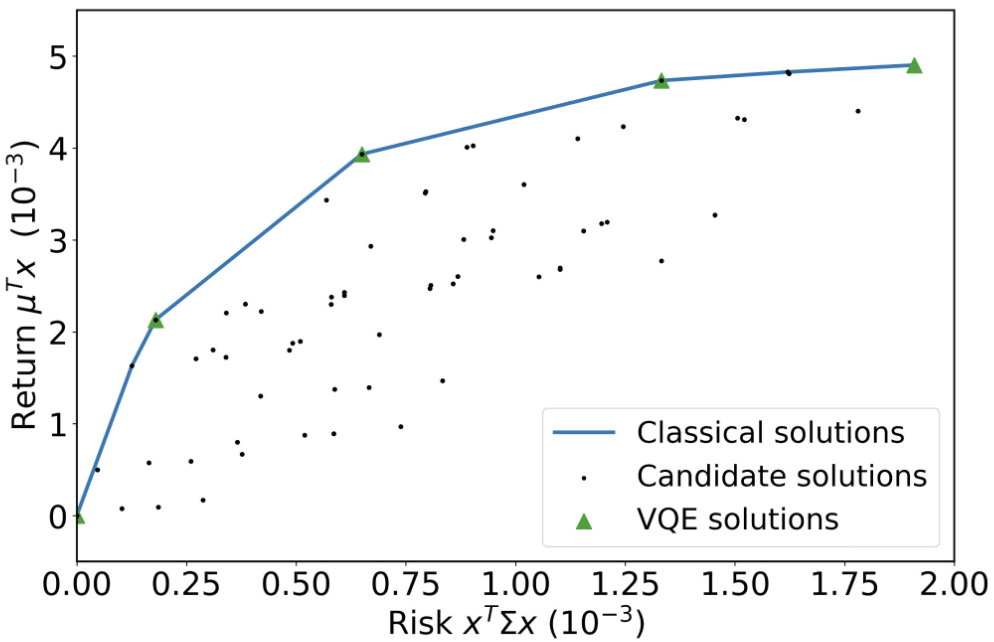
\includegraphics[width=0.8\linewidth]{EfficientFrontier_VQE.png}
    \caption{Beispiel einer Efficient Frontier in der Portfolio-Optimierung (simuliertes 6-Asset-Portfolio). Die blaue Kurve zeigt die optimale Risiko-Rendite-Kurve (klassische Exhaustivsuche), die grünen Dreiecke markieren Lösungen des Quantum-VQE-Algorithmus. Man sieht, dass die Quantenlösungen die Effizienzgrenze eng nachzeichnen (Rendite $\mu^T x$ und Risiko $x^T \Sigma x$ sind in willkürlichen Einheiten). (vgl. \cite[Abb. 8]{egger_quantum_2020}}
    \label{fig:efficient_frontier_vqe}
\end{figure}


Abb. \ref{fig:efficient_frontier_vqe} illustriert, dass bereits heutige gate-basierte Quantenalgorithmen wie der VQE in der Lage sind, für kleine Portfolios (hier ein simuliertes 6-Asset-Portfolio) ähnlich effiziente Lösungen wie klassische Exhaustivsuche zu erzeugen. Die grünen Dreiecke zeigen, dass die vom VQE generierten Lösungen eng entlang der klassischen Efficient Frontier liegen. Die zugrundeliegende Studie von Egger et al. (2020) verdeutlicht das Potenzial quantenbasierter Optimierung in Kombination mit VQE, insbesondere für risikoertragsbasierte Portfolioentscheidungen. 

Die zugrunde liegende Studie von Egger et al. (2020) demonstriert damit erfolgreich die prinzipielle Machbarkeit dieser Methode auf simulierten Quantencomputern. Einschränkungen bestehen jedoch weiterhin in Bezug auf Skalierbarkeit, da größere Portfolios tiefere Schaltkreise und längere Optimierung erfordern.
 
Bereits weitere Studien stehen im Einklang mit den Ergebnissen von Egger, und zeigen, dass unter kontrollierten Bedingungen bereits vielversprechende Ergebnisse erzielt werden können. So testeten mehrere Arbeiten die Wirksamkeit von VQE-Pipelines. Die Ergebnisse lieferten, dass der VQE auf einem 5-Qubit-Gerät eine fast identische Lösung zum klassischen Optimum generieren konnte. Die Qualität der Lösung variierte jedoch mit der Qualität des Quantenchips. Größere und weniger von Rausch behaftete Geräte lieferten verbesserte Ergebnisse als kleinere. Somit schmälern Rauschen und die begrenzte Qubit-Zahlen zwar noch den Nutzen, obwohl die Algorithmen prinzipiell eine optimale Lösung bieten (vgl. \cite{buonaiuto_best_2023}).
Der Einsatz von QAOA mit der Fixierung der Anzahl der enthaltenen Assets zeigte, dass die Anzahl benötigter Quantengatter und Messungen, die für mittlere Problemgrößen benötigt werden, die NISQ-Geräte an ihre Grenzen bringt. Für kleinere Portfolios konnten jedoch annähernd optimale Ergebnisse erzielt werden (vgl. \cite{brandhofer_benchmarking_2022}).
 
Beide Ansätze QAOA/VQE glänzen in Ihrer Flexibilität. Es können leichter zusätzliche Nebenbedingungen eingebaut und dynamische Portfolio-Probleme formuliert werden. Nachteile spiegeln sich in der Limitation durch Rauschen und Dekohärenz wider, die ohne notwendige Fehlerkorrektur nicht behoben werden können. Aufgrund dieser Einschränkungen bleiben die Anwendungen der gate-basierten Ansätze noch auf rein simulierter Ebene oder auf kleinen Hardware-Experimenten beschränkt(vgl. \cite{buonaiuto_best_2023}).


\section{Grundlegende Technologien}

Quantencomputer beruhen auf unterschiedlichen technologischen Prinzipien, die jeweils eigene algorithmische Strategien erfordern. Neben gate-basierten Universalarchitekturen existieren spezialisierte Modelle wie Quantum Annealing oder variationale Hybridverfahren, die auf bestimmte Problemklassen zugeschnitten sind.

Gate-basierte Quantencomputer operieren auf Basis quantenmechanischer Schaltkreise. Diese Architekturen ermöglichen insbesondere die Implementierung sogenannter Variationsalgorithmen, bei denen ein parametrischer Quantenschaltkreis durch einen klassischen Optimierer iterativ angepasst wird, um eine Zielfunktion zu minimieren oder zu maximieren. Zu den bekanntesten Verfahren dieser Art zählen der Quantum Approximate Optimization Algorithm (QAOA) und der Variational Quantum Eigensolver (VQE), die beide vor allem in der Portfoliooptimierung Anwendung finden und eine geeignete Problemformulierung in Form eines Ising-Hamiltonians voraussetzen (vgl. \cite{brandhofer_benchmarking_2022, buonaiuto_best_2023}). Ein weiteres wichtiges Verfahren ist Quantum Amplitude Estimation (QAE), das für quantenbasierte Monte-Carlo-Simulationen konzipiert wurde (vgl. \cite{egger_quantum_2020}).

Ergänzend zu diesen gate-basierten Methoden existieren adiabatische Verfahren wie das Quantum Annealing, das auf der sukzessiven Anpassung eines Hamiltonians beruht. Quantum Annealing eignet sich insbesondere für kombinatorische Optimierungsprobleme und verfolgt einen grundsätzlich anderen Lösungsansatz, der auf physikalischer Energieabsenkung basiert, anstatt auf diskreter Gate-Manipulation. Gerade im Finanzkontext zeigt sich eine wachsende Komplementarität beider Paradigmen: Während gate-basierte Verfahren zunehmend für simulations- und schätzbasierte Anwendungen wie Risikomodellierung und Optionsbewertung eingesetzt werden, zeigt Quantum Annealing Potenzial bei der effizienten Lösung von diskreten Optimierungsproblemen wie etwa der Portfoliozusammensetzung.

Dieses Kapitel gibt einen systematischen Überblick über die zentralen technologischen Ansätze und Quantenalgorithmen. Im Fokus stehen deren Funktionsprinzipien, technische Voraussetzungen sowie typische Einsatzbereiche. Ziel ist es, die strukturelle Vielfalt aktueller Quantencomputing-Ansätze herauszuarbeiten und deren Relevanz für verschiedene Anwendungsszenarien einzuordnen.

Zu den derzeit zentralen quantenbasierten Methoden im Finanzkontext gehören:

\begin{itemize}
\item Quantum Annealing (QA) – (Adiabatisches Verfahren)
\item Quantum Approximate Optimization Algorithm (QAOA) – (Gate-basierter Algorithmus)
\item Variational Quantum Eigensolver (VQE) – (Gate-basierter Algorithmus)
\item Quantum Amplitude Estimation (QAE) – (Gate-basierter Algorithmus)
\end{itemize}

Die folgenden Abschnitte analysieren diese Technologien aus technischer Perspektive. Sie zeigen, welche Stärken und Schwächen mit den jeweiligen Ansätzen verbunden sind und welche praktischen Voraussetzungen für deren erfolgreichen Einsatz im Finanzwesen erfüllt sein müssen.

\subsection{Quantum Annealing (QA)}

\subparagraph{Herkunft und Entwicklung}
Quantum Annealing (QA) ist ein quantenmechanisches Optimierungsverfahren, das auf dem Konzept der adiabatischen Quantenberechnung basiert. Die Idee wurde Anfang der 2000er-Jahre insbesondere durch Farhi et al. und D-Wave Systems weiterentwickelt und kommerzialisiert (vgl. \cite{orus_quantum_2019}). Während universelle Quantencomputer auf Gattermodellen beruhen, fokussiert sich QA auf die Lösung kombinatorischer Optimierungsprobleme durch sukzessive Energie-Minimierung in einem physikalischen System.

\subparagraph{Grundidee und Aufbau}
QA nutzt quantenmechanische Effekte wie Superposition und insbesondere Tunneling, um das globale Minimum einer Zielfunktion zu finden. Das Verfahren startet mit einem bekannten Anfangszustand (Anfangshamiltonian) und transformiert diesen langsam in den Zielzustand (Problemhamiltonian), wobei das System idealerweise stets im Grundzustand bleibt. Das zugrundeliegende Optimierungsproblem wird in ein sogenanntes \emph{Quadratic Unconstrained Binary Optimization} (QUBO) oder Ising-Modell übersetzt (vgl. \cite{orus_quantum_2019, mugel_dynamic_2022}).

\subparagraph{Technologische Basis}
Die Technologie basiert auf dem adiabatischen Theorem: Wird ein System hinreichend langsam verändert, verbleibt es mit hoher Wahrscheinlichkeit im Grundzustand (vgl. \cite{orus_quantum_2019}). Zur Umsetzung wird die Problemstruktur als QUBO-Modell kodiert, wobei binäre Variablen Entscheidungsoptionen (z.\,B. Asset-Auswahl) und deren Wechselwirkungen Risiken, Renditen oder Nebenbedingungen repräsentieren. Die physische Umsetzung erfolgt auf Hardware wie dem D-Wave-Quantenprozessor, wobei Qubits binären Variablen und Kopplungen den Interaktionen entsprechen (vgl. \cite{mugel_dynamic_2022}).

\subparagraph{Algorithmisches Vorgehen}
Zu Beginn befindet sich das System in einem leicht vorbereitbaren Grundzustand. Während des Annealing-Prozesses wird der Hamiltonian kontinuierlich in Richtung des Problems deformiert. Wenn dieser Übergang langsam genug erfolgt, bleibt das System im energetischen Minimum, dem optimalen Lösungskandidaten (vgl. \cite{orus_quantum_2019}). Dieses Vorgehen erlaubt es, auch in hochdimensionalen Problemräumen durch Quanten-Tunneling lokale Minima zu überwinden und globale Lösungen zu erreichen (vgl. \cite{mugel_dynamic_2022, rosenberg_finding_2016}).

\subparagraph{Modellierungsvoraussetzungen}
Eine Voraussetzung für QA ist die Transformation des Problems in eine QUBO-Form. Für viele finanzielle Anwendungen, insbesondere Portfoliooptimierung, ist dies gut möglich, da viele Constraints und Zielfunktionen binär darstellbar sind (vgl. \cite{mugel_dynamic_2022}). Einschränkungen ergeben sich jedoch bei komplexen, nichtlinear verknüpften Nebenbedingungen, deren QUBO-Formulierung zusätzlicher Modellierungsarbeit bedarf (vgl. \cite{sakuler_real-world_2025}).

\subparagraph{Chancen und Stärken}
QA bietet insbesondere bei kombinatorischen, binären Problemen eine attraktive Alternative zu klassischen Heuristiken. Vorteile sind die natürliche Hardware-Umsetzung auf spezialisierten Systemen wie D-Wave, die Fähigkeit zur Überwindung lokaler Minima durch Tunneling sowie eine schnelle Konvergenz bei kleinen bis mittelgroßen Problemgrößen (vgl. \cite{mugel_dynamic_2022, sakuler_real-world_2025}). Zudem zeigt sich in Studien, dass QA insbesondere bei realitätsnahen Portfolios mit echten Marktdaten effiziente Lösungen liefern kann (vgl. \cite{mugel_dynamic_2022}).

\subparagraph{Grenzen und Herausforderungen}
Ein zentrales Problem besteht in der begrenzten Skalierbarkeit aktueller Systeme: Sowohl die Anzahl als auch die Konnektivität der Qubits limitiert die Größe und Komplexität der darstellbaren Probleme (vgl. \cite{sakuler_real-world_2025}). Auch ist die Einbettung realer Constraints in die QUBO-Form nicht trivial und verlangt sorgfältiges Penalty-Tuning. Zudem ist die aktuelle Hardware noch anfällig für Rauschen, was insbesondere bei tiefer „Temperatur“ zu Fehlern führen kann (vgl. \cite{rosenberg_finding_2016, sakuler_real-world_2025}).

\subsection{Gate-basierte Ansätze (QAOA und VQE)}

Gate-basierte Quantencomputer arbeiten auf Basis von quantenmechanischen Schaltkreisen. Diese Systeme ermöglichen die Implementierung sogenannter Variationsalgorithmen, bei denen ein parametrischer Quantenschaltkreis durch einen klassischen Optimierer so angepasst wird, dass eine Zielfunktion minimiert oder maximiert wird. Zu den bekanntesten Methoden gehören der Quantum Approximate Optimization Algorithm (QAOA) und der Variational Quantum Eigensolver (VQE) (vgl. \cite{buonaiuto_best_2023, brandhofer_benchmarking_2022}). Beide Verfahren finden Anwendung in der Portfoliooptimierung, erfordern jedoch eine geeignete Problemformulierung in Form eines Ising-Hamiltonians.

\subsubsection{Quantum Approximate Optimization Algorithm (QAOA)}

\subparagraph{Herkunft und Entwicklung}
QAOA wurde ursprünglich 2014 von Farhi et al. entwickelt (vgl. \cite{farhi_quantum_2014}) und stellt eine hybride Methode dar, die speziell für kombinatorische Optimierungsprobleme konzipiert wurde. Im Gegensatz zu Quantum Annealing arbeitet QAOA nicht auf einem physikalisch kontinuierlichen Prozess, sondern diskret über parametrische Gate-Schaltungen. Es zählt zu den vielversprechendsten Algorithmen für sogenannte Noisy Intermediate-Scale Quantum (NISQ)-Geräte.

\subparagraph{Grundidee und Aufbau}
Der QAOA-Ansatz kombiniert zwei zentrale Operationen: eine Phasenoperation basierend auf dem Problemhamiltonian und eine Mischoperation über den sogenannten Mixer-Hamiltonian. Durch abwechselnde Anwendung dieser beiden Operatoren und Variation der Parameter wird ein Quantenzustand erzeugt, der eine möglichst hohe Wahrscheinlichkeit hat, die optimale Lösung zu repräsentieren (vgl. \cite{brandhofer_benchmarking_2022}).

\subparagraph{Technologische Basis}
Für QAOA muss das Optimierungsproblem binär formuliert und in ein Ising-Modell überführt werden. Dabei codieren Qubit-Zustände Entscheidungsvariablen, während Kopplungsterme die Interaktionen (z.\,B. Risiko-Rendite) abbilden. Die Implementierung erfolgt auf gate-basierten Quantenprozessoren, typischerweise innerhalb von Frameworks wie Qiskit oder Cirq (vgl. \cite{buonaiuto_best_2023}).

\subparagraph{Algorithmisches Vorgehen}
Der Algorithmus initialisiert einen Quantenzustand (meist im Gleichgewichtszustand) und führt anschließend $p$-mal abwechselnd zwei Schichten aus: eine Phase-Schicht $U_C(\gamma)$, die auf dem Problemhamiltonian basiert, und eine Mixer-Schicht $U_B(\beta)$, die eine Rotation im Zustandsspektrum bewirkt. Nach jeder Iteration werden die Parameter $\gamma$ und $\beta$ durch einen klassischen Optimierer angepasst. Ziel ist es, die Messwahrscheinlichkeit für optimale Lösungen zu maximieren (vgl. \cite{brandhofer_benchmarking_2022}).

\subparagraph{Voraussetzungen und Modellierung}
Ein geeignetes QUBO- oder Ising-Modell ist Voraussetzung. Besonders die Abbildung harter Constraints stellt eine Herausforderung dar, da diese mit Penalty-Terms implementiert werden müssen. Spezialisierte Mixer können hierbei die Ergebnisqualität und Konvergenz verbessern, wie etwa in der Studie von Brandhofer et al. gezeigt (vgl. \cite{brandhofer_benchmarking_2022}).

\subparagraph{Chancen und Stärken}
QAOA ist besonders gut geeignet für kombinatorische Probleme mit binärer Struktur. Die geringe Tiefe der Schaltungen macht es für NISQ-Hardware attraktiv. Die Möglichkeit, domänenspezifische Mixer zu integrieren, bietet zusätzliche Flexibilität (vgl. \cite{brandhofer_benchmarking_2022}).

\subparagraph{Grenzen und Herausforderungen}
Die praktische Leistungsfähigkeit ist stark von der Wahl der Parameter, der Problemgröße und dem Hardware-Backend abhängig. Mit zunehmender Tiefe steigt die Empfindlichkeit gegenüber Rauschen. Zudem erfordert die Parametereinstellung oft umfangreiche Hyperparameter-Tuning-Prozesse (vgl. \cite{buonaiuto_best_2023}).

\subsubsection{Variational Quantum Eigensolver (VQE)}

\subparagraph{Herkunft und Entwicklung}
Der Variational Quantum Eigensolver (VQE) wurde 2014 eingeführt und war eine der ersten Methoden zur Nutzung von NISQ-Geräten für Optimierungsprobleme in Physik und Chemie. Anders als QAOA richtet sich VQE nicht ausschließlich an kombinatorische Probleme, sondern zielt allgemein auf das Auffinden von Grundzuständen komplexer Hamiltonians ab (vgl. \cite{buonaiuto_best_2023}).

\subparagraph{Grundidee und Aufbau}
VQE basiert auf dem variationalen Prinzip der Quantenmechanik: Der Erwartungswert des Hamiltonians wird auf einem parametrischen Quantenzustand minimiert. Dieser Zustand wird durch einen sogenannten Ansatz erzeugt, ein vorgegebener Schaltkreis mit variierbaren Parametern. Die Optimierung erfolgt iterativ mit Hilfe eines klassischen Optimierungsalgorithmus (vgl. \cite{buonaiuto_best_2023}).

\subparagraph{Technologische Basis}
Das zugrunde liegende Optimierungsproblem wird zunächst in ein QUBO-Modell transformiert, welches dann in ein Ising-Hamiltonian überführt wird. Über die Wahl des Ansatzes und die Operatorbasis (z.\,B. Pauli-Zerlegung) wird der Hamiltonian auf einem realen Quantenprozessor gemessen. Die Messwerte dienen als Eingabe für die klassische Optimierung.

\subparagraph{Algorithmisches Vorgehen}
VQE setzt auf eine wiederholte Schleife aus Quanten- und Klassikprozessor: Zunächst wird der parametrische Schaltkreis vorbereitet und gemessen. Dann schätzt der klassische Teil den Erwartungswert des Hamiltonians und passt die Parameter des Ansatzes an. Dieser Vorgang wird solange wiederholt, bis eine Konvergenz zum Energie-Minimum erreicht ist (vgl. \cite{buonaiuto_best_2023}).

\subparagraph{Voraussetzungen und Modellierung}
Für die Portfoliooptimierung wird das ursprüngliche Problem zunächst in ein binäres Quadratic Programming-Modell transformiert. Constraints wie Budgetgrenzen werden in die Zielfunktion eingebettet, indem sie als Strafterme gewichtet werden. Die Effizienz hängt stark von der richtigen Wahl des Ansatzes, des Optimierers sowie der Penalty-Koeffizienten ab (vgl. \cite{buonaiuto_best_2023}).

\subparagraph{Chancen und Stärken}
VQE zeigt große Flexibilität hinsichtlich der Wahl des Ansatzes und eignet sich besonders gut für kontinuierliche oder strukturierte Optimierungsprobleme. Studien zeigen, dass bei richtiger Parametrisierung auf realer Hardware (z.\,B. IBM Q) sehr gute Ergebnisse erzielt werden können, auch ohne aufwändige Fehlerkor


\subsection{Quantum Amplitude Estimation (QAE)}

\subparagraph{Herkunft und Entwicklung}
Quantum Amplitude Estimation (QAE) wurde im Jahr 2000 von Brassard et al. eingeführt und gehört zur Klasse der quantenmechanischen Algorithmen, die auf der Grover-Suche aufbauen (vgl. \cite{quantumjournal2020}). Das Ziel war, klassische Monte-Carlo-Verfahren durch quadratische Geschwindigkeitsvorteile zu übertreffen. Im Unterschied zu Ansätzen wie Quantum Annealing oder VQE, die auf Optimierung abzielen, adressiert QAE das Problem der präzisen Erwartungsschätzung – ein zentraler Aspekt in stochastischen Simulationen.

\subparagraph{Grundidee und Aufbau}
QAE zielt darauf ab, Wahrscheinlichkeiten bzw. Erwartungswerte effizient zu schätzen. Dazu nutzt es die quantenmechanische Superposition sowie Amplitudeninterferenz, um Zustände mit hoher Relevanz zu verstärken. Die Wahrscheinlichkeit für das Auftreten eines gewünschten Ergebnisses wird dabei indirekt über Messungen in speziell vorbereiteten Zuständen ermittelt. Im Gegensatz zu klassischen Monte-Carlo-Verfahren, bei denen zur Erreichung einer Genauigkeit $\varepsilon$ eine Komplexität von $O(1/\varepsilon^2)$ notwendig ist, erreicht QAE dies mit nur $O(1/\varepsilon)$ Abfragen (vgl. \cite{quantumjournal2020, rebentrost_quantum_2018}).

\subparagraph{Technologische Basis}
QAE kombiniert mehrere quantentechnische Bausteine: Vorbereitung eines Superpositionszustands, Anwendung einer Oracle-Funktion zur Kodierung des Problems, kontrollierte Grover-Operatoren zur Amplitudenverstärkung sowie eine abschließende Quanten-Fourier-Transformation zur Schätzung der Zielamplitude (vgl. \cite{martin2022}). Die Berechnungen erfolgen auf gate-basierten Quantencomputern. Die zugrunde liegende Struktur ist auf tiefe und komplexe Quantenschaltkreise angewiesen, was besondere Anforderungen an Kohärenzzeiten und Fehlerkorrektur stellt.

\subparagraph{Algorithmisches Vorgehen}
Im ersten Schritt wird ein Zustand vorbereitet, der die Lösungswahrscheinlichkeit in seiner Amplitude trägt. Anschließend erfolgt die wiederholte Anwendung des Grover-Operators, der die Wahrscheinlichkeit des Zielzustands periodisch verstärkt. Die Anzahl der Grover-Schritte variiert kontrolliert, sodass über Quanteninterferenz ein Phasenintervall entsteht, welches über die inverse Quanten-Fourier-Transformation präzise ausgelesen werden kann. Das Ergebnis ist eine Schätzung der Zielwahrscheinlichkeit mit quadratisch höherer Effizienz im Vergleich zur klassischen Simulation (vgl. \cite{quantumjournal2020, martin2022}).

\subparagraph{Voraussetzungen und Modellierung}
Damit QAE zur Anwendung kommen kann, muss das zugrunde liegende Problem so formuliert werden, dass es sich als Wahrscheinlichkeitsverteilung über einem Quantenzustand ausdrücken lässt. In der Praxis bedeutet dies, dass die Bewertung (z.\,B. eines Finanzinstruments) als Erwartungswert über Zufallsvariablen formuliert sein muss. Die Komplexität der Problemabbildung liegt vor allem in der Konstruktion des Orakels und der effizienten Kodierung der stochastischen Prozesse in die Amplituden (vgl. \cite{rebentrost_quantum_2018}).

\subparagraph{Chancen und Stärken}
QAE eignet sich besonders für Probleme, bei denen Erwartungswerte über große Stichprobenräume geschätzt werden müssen, etwa bei der Bewertung komplexer, pfadabhängiger Optionen oder der Berechnung von Value-at-Risk (VaR) (vgl. \cite{orus_quantum_2019}). Die quadratische Beschleunigung gegenüber Monte-Carlo-Methoden führt zu erheblichen Effizienzgewinnen. Studien zeigen, dass bereits bei moderaten Genauigkeitsanforderungen signifikante Reduktionen im Rechenaufwand möglich sind (vgl. \cite{rebentrost_quantum_2018, egger_quantum_2020}). Darüber hinaus eröffnet QAE neue Möglichkeiten zur Modellierung realitätsnaher Szenarien, die mit klassischen Methoden bislang nicht praktikabel waren.

\subparagraph{Grenzen und Herausforderungen}
Die größte Herausforderung in der praktischen Umsetzung liegt in den hardwareseitigen Anforderungen. QAE benötigt tiefe Quantenschaltkreise, die auf heutigen NISQ-Geräten aufgrund limitierter Qubit-Anzahl, kurzer Kohärenzzeiten und hoher Fehlerraten nur schwer zuverlässig realisierbar sind (vgl. \cite{bouland_prospects_2020, martin2022}). Auch die Konstruktion eines effizienten Orakels ist nicht trivial und hängt stark vom Anwendungsfall ab. Darüber hinaus ist die statistische Robustheit des Algorithmus empfindlich gegenüber Messfehlern, was die praktische Anwendbarkeit einschränkt.

\subparagraph{Praktische Perspektiven und Entwicklungen}
Trotz dieser Hürden gibt es vielversprechende Entwicklungen: Kooperationen wie jene zwischen JPMorgan und IBM oder Forschungsprojekte von Google zeigen, dass QAE in der Finanzbranche ernsthaft evaluiert wird (vgl. \cite{egger_quantum_2020}). Erste Proof-of-Concepts für die Optionsbewertung auf simulierten und realen Quantenplattformen sind bereits veröffentlicht worden. Die zukünftige Skalierung hängt maßgeblich von Fortschritten in der Hardwareentwicklung und der Fehlerkorrektur ab.

\subsection{Vergleich der analysierten Technologien}

Zur Einordnung der vorgestellten quantenmechanischen Verfahren: Quantum Annealing (QA), Quantum Approximate Optimization Algorithm (QAOA), Variational Quantum Eigensolver (VQE) sowie Quantum Amplitude Estimation (QAE) bietet sich ein zweistufiger Vergleich an. Zunächst erfolgt ein technologischer Vergleich anhand funktionaler und struktureller Merkmale, gefolgt von einer allgemeinen Bewertung hinsichtlich Reifegrad und industrieller Perspektiven.

\subsubsection*{Technologischer Vergleich}

\begin{table}[H]
\centering
\caption{Technologisch-struktureller Vergleich der Methoden}
\renewcommand{\arraystretch}{1.2}
\begin{tabular}{|p{0.26\linewidth}|p{0.18\linewidth}|p{0.18\linewidth}|p{0.18\linewidth}|p{0.18\linewidth}|}
\hline
\textbf{Kriterium} & \textbf{QA} & \textbf{QAOA} & \textbf{VQE} & \textbf{QAE} \\
\hline
Plattform & Adiabatisch & Gate-basiert & Gate-basiert & Gate-basiert \\
\hline
Zieltyp & Optimierung & Optimierung & Optimierung & Schätzung \\
\hline
Formulierung & QUBO/Ising & Ising-Modell & Hamiltonian & Orakel \\
\hline
Ressourcen & Kopplungen & Tiefe Gates & Variabler Ansatz & QFT, Gates \\
\hline
Struktur & Hardware-nah & Alternierend & Flexibel & Interferenz \\
\hline
Fehlersensitivität & Gering & Hoch & Hoch & Sehr hoch \\
\hline
Qubitbedarf & Niedrig & Mittel & Mittel & Hoch \\
\hline
\end{tabular}
\end{table}

\subsubsection*{Bewertung und Analyse: Technologisch-struktureller Vergleich}

\paragraph{Analyse ausgewählter Aspekte}

Bereits der erste Eintrag zeigt eine klare Trennung: Während Quantum Annealing (QA) auf einem adiabatischen Hardwaremodell basiert, setzen alle anderen Verfahren auf gate-basierte Systeme. Dies macht QA besonders hardware-nah und ressourcenschonend, da es keine komplexen Schaltungen benötigt (vgl. \cite{orus_quantum_2019, mugel_dynamic_2022}). Die Kopplungen zwischen Qubits übernehmen direkt die Problemstruktur. Im Gegensatz dazu erfordern QAOA, VQE und QAE komplexe Gate-Sequenzen, die eine präzise Steuerung voraussetzen (vgl. \cite{buonaiuto_best_2023}).

Ein auffälliger Unterschied zeigt sich beim Zieltyp: Während QA, QAOA und VQE für Optimierungsprobleme entwickelt wurden, dient QAE der Schätzung von Wahrscheinlichkeiten, etwa bei Monte-Carlo-Simulationen oder Value-at-Risk-Modellen (vgl. \cite{rebentrost_quantum_2018, quantumjournal2020}). Daraus ergeben sich tiefgreifende Unterschiede in der Struktur und Ressourcennutzung. Insbesondere QAE benötigt tiefe, kontrollierte Quantenschaltkreise inklusive Quanten-Fourier-Transformation, was es zu einer der anspruchsvollsten Methoden macht (vgl. \cite{martin2022}).

Der Punkt „Struktur“ verdeutlicht, wie unterschiedlich die Algorithmen designt sind: QAOA arbeitet mit alternierenden Operatoren (Problem- und Mixer-Gates), während VQE auf einen frei wählbaren Ansatz basiert, der auf die Hardware optimiert sein kann (vgl. \cite{brandhofer_benchmarking_2022}). QA hingegen nutzt eine kontinuierliche Energielandschaft, was eine ganz andere physikalische Interpretation erlaubt.

In Bezug auf Fehlertoleranz und Qubitbedarf zeigen sich wieder zwei Extreme: QA benötigt vergleichsweise wenige Qubits mit eingeschränkter Konnektivität, ist dafür aber relativ robust gegenüber Fehlern (vgl. \cite{sakuler_real-world_2025}). QAE hingegen ist stark fehleranfällig und benötigt eine hohe Zahl kohärenter Qubits (vgl. \cite{bouland_prospects_2020}), was es aktuell noch limitiert.

Der technologische Vergleich zeigt klar, dass sich die Verfahren nicht nur im Ziel, sondern auch in ihrer Hardware- und Ressourcenausrichtung stark unterscheiden. Während QA eine spezialisierte, robuste Lösung für bestimmte Optimierungsprobleme bietet, sind VQE, QAOA und QAE flexibler, aber in ihrer aktuellen Form noch stark abhängig von der Hardwareentwicklung.

\subparagraph{Legende der Einstufungen}

\begin{itemize}
    \item \textbf{hoch}: Verfahren ist etabliert, gut erforscht oder praxistauglich.
    \item \textbf{mittel}: Verfahren ist teilweise anwendbar, unterliegt aber Einschränkungen.
    \item \textbf{niedrig}: Aktuell kaum praktikabel oder nur experimentell umsetzbar.
    \item \textbf{aufstrebend / wachsend / sehr hoch}: Verfahren mit stark wachsendem Potenzial, aber begrenztem Stand heute.
\end{itemize}

\subsubsection*{Reifegrad und Anwendungsperspektiven}

\begin{table}[H]
\centering
\caption{Bewertung der Verfahren nach Reifegrad und industrieller Perspektive}
\renewcommand{\arraystretch}{1.2}
\begin{tabular}{|p{0.24\linewidth}|p{0.19\linewidth}|p{0.19\linewidth}|p{0.19\linewidth}|p{0.19\linewidth}|}
\hline
\textbf{Kriterium} & \textbf{QA} & \textbf{QAOA} & \textbf{VQE} & \textbf{QAE} \\
\hline
Reifegrad & hoch & mittel & mittel & niedrig \\
\hline
Hardware-Kompatibilität & hoch & mittel & mittel & niedrig \\
\hline
Industrielle Relevanz & hoch & mittel & mittel & aufstrebend \\
\hline
Skalierbarkeit & gering & mittel & mittel & gering \\
\hline
Fehlerkorrektur & gering & hoch & hoch & sehr hoch \\
\hline
Forschungstiefe & hoch & hoch & sehr hoch & wachsend \\
\hline
Zukunftspotenzial & mittel & hoch & hoch & sehr hoch \\
\hline
\end{tabular}
\end{table}


\subsubsection*{Bewertung und Analyse: Reifegrad und Anwendungsperspektiven}

Die Tabelle gibt einen überblicksartigen Vergleich der vier betrachteten quantenmechanischen Verfahren entlang zentraler Anwendungskriterien. Dabei geht es weniger um eine vollständige Bewertung, sondern vielmehr um eine Orientierung entlang von Stärken und Schwächen in Bezug auf praktische Umsetzbarkeit, Forschungsstand und Zukunftspotenzial.



\paragraph{Analyse ausgewählter Kriterien}

Besonders auffällig ist die hohe Bewertung von Quantum Annealing (QA) im Hinblick auf den technologischen Reifegrad und die praktische Umsetzbarkeit. Diese Einschätzung basiert auf der industriellen Nutzung durch Anbieter wie D-Wave sowie reale Anwendungen etwa in der Portfolio- oder Supply-Chain-Optimierung (vgl. \cite{mugel_dynamic_2022, sakuler_real-world_2025}). Dennoch zeigt QA gleichzeitig eine \emph{geringe Skalierbarkeit}, was mit der begrenzten Qubit-Konnektivität aktueller Annealer zusammenhängt (vgl. \cite{sakuler_real-world_2025}).

Quantum Amplitude Estimation (QAE) weist ein gegenteiliges Profil auf: Es besitzt ein \emph{sehr hohes Zukunftspotenzial}, kann aber derzeit aufgrund der tiefen Schaltkreise und des Bedarfs an Fehlerkorrektur kaum praktisch eingesetzt werden (vgl. \cite{bouland_prospects_2020, martin2022}). Die „niedrig“-Bewertung bei Umsetzbarkeit entspricht dem aktuellen Stand auf NISQ-Geräten.

Variational Quantum Eigensolver (VQE) wird in der Literatur häufig für chemische und finanzielle Modellierungen eingesetzt, insbesondere auf IBM-Q-Systemen (vgl. \cite{buonaiuto_best_2023}). Die Kombination aus mittelmäßigem Reifegrad und hohem Forschungsstand ist hier konsistent: Die Methode ist anpassbar, aber hardwareintensiv.

Der QAOA-Ansatz liegt in fast allen Dimensionen zwischen QA und VQE, was durch seine modulare Gate-Struktur begründet ist. Studien zeigen jedoch, dass bei sorgfältiger Parametrisierung und Spezialisierung deutliche Fortschritte erzielt werden können (vgl. \cite{brandhofer_benchmarking_2022}).

Zusammenfassend zeigt sich, dass aktuell nur QA als produktionsnah gelten kann, während QAOA und VQE im mittleren Reifegrad operieren. QAE hingegen steht als vielversprechender, aber technisch herausfordernder Spezialfall am Anfang seiner Entwicklung.



\section{Unternehmen und Akteure}
Quantencomputing hat sich in den vergangenen Jahren zu einem zentralen Innovationsfeld entwickelt, in dem sowohl große Technologiekonzerne als auch spezialisierte Unternehmen aus dem Finanzsektor aktiv sind. Diese Akteure tragen wesentlich zur technologischen Entwicklung, praktischen Anwendung und breiteren Implementierung quantenbasierter Lösungen bei.

\subsection{Allgemeine Akteure im Quantenbereich}

Große Technologiekonzerne prägen die allgemeine Entwicklung des Quantencomputings maßgeblich. IBM bietet mit IBM Quantum Experience eine cloud-basierte Plattform an, die Zugang zu gate-basierten Quantencomputern mit bis zu 433 Qubits ermöglicht und Forschenden und Unternehmen erlaubt, ihre Algorithmen praktisch zu testen (vgl.\cite{IBM, 2023}). Google verfolgt ebenfalls einen gate-basierten Ansatz und erzielte mit dem Sycamore-Prozessor Quantum Supremacy, indem sie zeigten, dass Quantencomputer spezifische Rechenprobleme deutlich schneller lösen können als klassische Rechner (Vgl.\cite{arute_quantum_2019}). D-Wave hingegen verfolgt den Ansatz des Quantum Annealings, der sich insbesondere für kombinatorische Optimierungsprobleme eignet und bereits in Industrieanwendungen, z.B. im Logistik- und Finanzsektor, eingesetzt wird (vgl. \cite{Johson et al. 2011}).

\subsection{Spezifische Akteure im Finanzsektor}

Parallel zur allgemeinen technologischen Entwicklung haben zahlreiche Finanzinstitutionen das Potenzial von Quantencomputing erkannt und entwickeln gezielt anwendungsorientierte Lösungen. JP Morgan investiert gezielt in Projekte, die sowohl Quantum Annealing als auch gate-basierte Methoden einsetzen, um komplexe Optimierungsprobleme und Risikobewertungen zu verbessern. Ein Beispiel hierfür ist die Anwendung von Quantum Annealing zur Portfoliooptimierung, bei der signifikante Effizienzgewinne erzielt wurden (vgl.\cite{Herman et al., 2022}). Goldman Sachs konzentriert sich besonders auf quantenbasierte Monte-Carlo-Simulationen zur Verbesserung der Preisgestaltung und Risikomessung komplexer Finanzprodukte und hat erste Pilotprojekte mit gate-basierten Quantencomputern erfolgreich getestet (vgl.\cite{egger_quantum_2020}). Die spanische Bank BBVA arbeitet mit unterschiedlichen Technologiepartnern wie Multiverse Computing zusammen, um quantenbasierte Algorithmen für Handelsstrategien und Risikoanalysen zu erproben, was erste vielversprechende Ergebnisse hinsichtlich Geschwindigkeit und Genauigkeit gezeigt hat (vgl.\cite{orus_quantum_2019}).

Diese spezifischen Akteure spielen eine zentrale Rolle dabei, quantenbasierte Innovationen im Finanzwesen voranzutreiben, indem sie konkrete Anwendungsfälle entwickeln und gleichzeitig praktische Erfahrungen sammeln, die wiederum in die allgemeine technologische Weiterentwicklung zurückfließen.


\section{Zentrale Zukunftsprojekte und Forschungsinitiativen}

Der Fortschritt im Quantencomputing für Finanzanwendungen wird wesentlich durch spezifische Projekte und strategische Forschungsinitiativen geprägt. Diese konzentrieren sich auf die Entwicklung praxisnaher quantenbasierter Lösungen, speziell für Anwendungen im Finanzsektor. Im Folgenden werden zentrale Zukunftsprojekte ausführlich vorgestellt sowie deren Ziele, Inhalte und bisherigen Ergebnisse umfassend beschrieben.

\subsection{IBM Quantum Roadmap – Skalierung der Quantenhardware}

Die IBM Quantum Roadmap stellt ein langfristiges, strategisches Projekt dar, das sich auf die schrittweise Verbesserung und industrielle Skalierung von Quantenhardware konzentriert. IBM strebt dabei eine kontinuierliche Erhöhung der Anzahl und Qualität supraleitender Qubits an, mit dem Ziel, innerhalb der nächsten Jahre Quantenprozessoren mit Tausenden von Qubits bereitzustellen. Diese technologische Weiterentwicklung ist entscheidend, um komplexere Algorithmen mit praxisrelevanter Größenordnung durchführen zu können und somit den kommerziellen Einsatz in Bereichen wie Finanzdienstleistungen zu ermöglichen. Im Rahmen der Roadmap wurden bereits signifikante Fortschritte erzielt, darunter die Einführung von Quantenprozessoren mit mehreren hundert Qubits, die aktuell durch Cloud-Plattformen nutzbar sind (vgl.\cite{IBM Quantum, 2023}).

\subsection{NEASQC – Europäisches Projekt für NISQ-Anwendungen}

Das Projekt NEASQC (Next Applications of Quantum Computing) wird von der Europäischen Union im Rahmen des Programms Horizon 2020 finanziert und verfolgt das Ziel, Algorithmen und Anwendungen für NISQ-Geräte (Noisy Intermediate-Scale Quantum) zu entwickeln. Das Projekt adressiert praxisrelevante industrielle Anwendungen und konzentriert sich insbesondere auf Finanzanwendungen wie Monte-Carlo-Simulationen, Portfolioanalysen und die Hauptkomponentenanalyse (PCA). HSBC nimmt als Finanzakteur eine zentrale Rolle im Konsortium ein und validiert entwickelte quantenbasierte Methoden anhand konkreter bankwirtschaftlicher Szenarien. Das Projekt verfolgt einen offenen Ansatz und veröffentlicht die Algorithmen sowie Testumgebungen unter Open-Source-Lizenzen, um breitere industrielle Anwendbarkeit zu gewährleisten und Synergien zwischen Forschung und Industrie zu fördern \cite{(NEASQC, 2025; \cite{Manzano et al., 2024}).

\subsection{IBM Quantum Finance – Quantenalgorithmen für Risikoanalyse und Simulation}

Unter dem Titel „IBM Quantum Finance“ verfolgt IBM die Entwicklung spezifischer Quantenalgorithmen, die speziell für Anwendungen im Finanzsektor geeignet sind. Ein wesentlicher Schwerpunkt ist die Quantum Amplitude Estimation (QAE), welche Monte-Carlo-Simulationen stark beschleunigt und gleichzeitig Genauigkeitsgewinne ermöglicht. Konkret wird QAE bei der Bewertung komplexer Finanzinstrumente, der Risikomodellierung und der Berechnung von Risikokennzahlen wie dem Value at Risk (VaR) eingesetzt. IBM arbeitet hierbei eng mit Finanzinstituten wie JPMorgan Chase zusammen, um reale Finanzmodelle zu testen und ihre Ergebnisse direkt in die Praxis zu überführen. Erste Anwendungstests zeigen, dass Quantenverfahren deutliche Effizienz- und Präzisionsvorteile gegenüber klassischen Ansätzen bieten \cite({Larsson & Oosterlee, 2019; Moody’s, 2024}).

\subsection{D-Wave Portfolio Pilot – Portfoliooptimierung mittels Quantum Annealing}

D-Wave Systems betreibt das „D-Wave Portfolio Pilot“-Projekt, das speziell auf die Anwendung von Quantum Annealing-Technologie zur Portfoliooptimierung fokussiert ist. Ziel des Pilotprojekts ist es, Finanzunternehmen praktische Einblicke und konkrete Vorteile der Quantum-Annealing-Methode für die Lösung kombinatorischer Optimierungsprobleme wie etwa der optimalen Asset-Allokation zu verschaffen. Die Ergebnisse des Projekts belegen eine erheblich gesteigerte Effizienz und verbesserte Lösungsqualität gegenüber traditionellen Optimierungstechniken. Verschiedene Finanzunternehmen nutzen bereits die Technologie von D-Wave in Pilotprojekten, um reale Portfoliooptimierungen durchzuführen und konkrete Anwendungsszenarien zu validieren (Vgl.\cite{D-Wave Systems, 2023; Herman et al., 2022}).


\section{Bewertung der Anwendungsbereiche}

Auf Basis der in diesem Kapitel analysierten Anwendungsfelder erfolgt im Folgenden eine vergleichende Bewertung der drei zentralen Einsatzbereiche von Quantencomputing im Finanzwesen: Portfoliooptimierung, Optionsbewertung und Risikobemessung. Die Bewertung orientiert sich an fünf übergeordneten Kriterien: technologischer Reifegrad, wirtschaftliche Nutzbarkeit, gesellschaftlicher Nutzen, Forschungspotenzial sowie Risiken und ethische Implikationen.

Ziel dieser Gegenüberstellung ist es, die unterschiedlichen Entwicklungsstände, Chancen und Herausforderungen der betrachteten Anwendungsfelder systematisch einzuordnen. Dabei wird deutlich, in welchen Bereichen bereits erste praxisnahe Anwendungen existieren und wo insbesondere aus wissenschaftlicher Perspektive weiterführende Forschung notwendig ist, um das volle Potenzial quantenbasierter Methoden auszuschöpfen.

Die Bewertungen erfolgen auf einer qualitativen Skala von \emph{niedrig} über \emph{mittel} bis \emph{hoch} und dienen der vereinfachten Einordnung der jeweiligen Merkmalsausprägungen in den betrachteten Anwendungsfeldern.


\begin{table}[!htbp]
\centering
\renewcommand{\arraystretch}{1.5}
\begin{tabular}{|p{0.25\linewidth}|p{0.23\linewidth}|p{0.23\linewidth}|p{0.23\linewidth}|}
\hline
\textbf{Kriterium} & \textbf{Portfoliooptimierung} & \textbf{Optionsbewertung} & \textbf{Risikobemessung (VaR/CVaR)} \\
\hline
Technologischer Reifegrad & mittel & niedrig & niedrig \\
\hline
Marktrelevanz & hoch & hoch & sehr hoch \\
\hline
Gesellschaftlicher Nutzen & mittel & mittel & hoch \\
\hline
Forschungspotenzial & hoch & sehr hoch & sehr hoch \\
\hline
Risiken und Ethik & gering & mittel & hoch \\
\hline
\end{tabular}
\caption{Bewertung der drei Hauptanwendungsfelder von Quantencomputing im Finanzwesen}
\label{tab:anwendungsbewertung}
\end{table}


\subsection*{Erläuterung der Bewertungskriterien}

Im Folgenden werden die fünf Bewertungskriterien der Tabelle detailliert erläutert und jeweils für die drei Anwendungsfelder \textit{Portfoliooptimierung}, \textit{Optionsbewertung} und \textit{Risikobemessung (Value at Risk / Conditional Value at Risk)} eingeordnet.

\subsubsection*{Technologischer Reifegrad}

Die \textit{Portfoliooptimierung} weist den höchsten Reifegrad auf. Quantum Annealing wurde bereits in praktischen Studien erfolgreich angewendet (z.\,B.\ mit D-Wave-Systemen), insbesondere bei kleinen bis mittelgroßen Portfolios (vgl. \cite{rosenberg_finding_2016}), (vgl. \cite{mugel_dynamic_2022}). Gate-basierte Verfahren wie VQE wurden zudem erfolgreich simuliert (vgl. \cite{egger_quantum_2020}).

Die \textit{Optionsbewertung} ist in einem früheren Stadium. Zwar konnte Quantum Amplitude Estimation (QAE) auf realen Quantenchips wie IBM Tokyo erfolgreich getestet werden, etwa zur Bewertung von Barrier-Optionen (vgl. \cite{stamatopoulos_option_2020}), doch das effiziente Laden von Wahrscheinlichkeitsverteilungen bleibt eine Herausforderung.

Für die \textit{Risikobemessung} (VaR/CVaR) existieren erste Proof-of-Concepts wie bei Woerner und Egger (vgl. \cite{orus_quantum_2019}), jedoch ist die Skalierbarkeit auf realistische Portfolios bislang technisch limitiert. Die notwendige Datenkodierung erfordert komplexe Vorverarbeitung (vgl. \cite{zoufal_quantum_2019}).

\subsubsection*{Marktrelevanz / Wirtschaftliche Nutzbarkeit})

Die \textit{Portfoliooptimierung} ist ökonomisch relevant für institutionelle Anleger, Robo-Advisors und Asset Manager. Optimierte Allokationen können direkte Renditeeffekte erzielen (vgl. \cite{sakuler_real-world_2025}), (vgl. \cite{mugel_dynamic_2022}).

Die \textit{Optionsbewertung} hat ebenso hohe wirtschaftliche Bedeutung, da Derivate eine zentrale Rolle im Risikomanagement und der Preisfindung an Finanzmärkten spielen (vgl. \cite{stamatopoulos_option_2020}).

Die \textit{Risikobemessung} besitzt die höchste Relevanz, da regulatorische Anforderungen (Basel III/IV) tägliche Berechnung von VaR und CVaR verlangen. Jede Effizienzsteigerung hat direkte Auswirkungen auf Kapitalanforderungen (vgl. \cite{orus_quantum_2019}), (vgl. \cite{bouland_prospects_2020}).

\subsubsection*{Gesellschaftlicher Nutzen}

Die \textit{Portfoliooptimierung} wirkt nur indirekt gesellschaftlich, etwa durch effizientere Kapitalmärkte und stabilere Anlagestrategien.

Bei der \textit{Optionsbewertung} ist der Nutzen ebenfalls mittelbar: Genauere Preisfindung verhindert Fehlbewertungen und trägt zur Marktstabilität bei (vgl. \cite{stamatopoulos_option_2020}).

Die \textit{Risikobemessung} hat den größten gesellschaftlichen Wert: Sie dient der Früherkennung systemischer Risiken und damit dem Schutz von Volkswirtschaften vor Finanzkrisen (vgl. \cite{orus_quantum_2019}), (vgl. \cite{zoufal_quantum_2019}).

\subsubsection*{Forschungspotenzial / Innovationsgrad}

Die \textit{Portfoliooptimierung} bleibt ein aktives Forschungsfeld: Neue hybride Algorithmen (z.\,B.\ QAOA mit Constraint-Encoding) bieten Raum für methodische Innovationen (vgl. \cite{buonaiuto_best_2023}).

Die \textit{Optionsbewertung} zeigt sehr hohe Innovationskraft: Die Kombination aus QAE, variationalen Methoden und qGANs zur Datenkodierung bietet vielfältige Ansätze für algorithmische Forschung (vgl. \cite{zoufal_quantum_2019}), (vgl. \cite{stamatopoulos_option_2020}).

Auch die \textit{Risikobemessung} ist forschungsintensiv. Sie vereint Themen wie Tail-Risiko, stochastische Prozesse und Quantum Machine Learning (vgl. \cite{egger_quantum_2020}), (vgl. \cite{martin2022}).

\subsubsection*{Risiken und ethische Implikationen}

Die \textit{Portfoliooptimierung} ist relativ risikoarm. Fehlentscheidungen betreffen vor allem institutionelle Investoren und lassen sich in Simulationen evaluieren (vgl. \cite{sakuler_real-world_2025}).

Die \textit{Optionsbewertung} birgt mittlere Risiken. Unzureichend getestete Modelle könnten Fehlbewertungen verursachen. Zudem ist die Nachvollziehbarkeit von QAE-Methoden begrenzt (vgl. \cite{stamatopoulos_option_2020}).

Die \textit{Risikobemessung} bringt die größten ethischen Herausforderungen mit sich. Fehlerhafte Modellierung von Extremszenarien kann zu systemischen Risiken führen. Die Black-Box-Natur mancher Quantenmodelle erschwert die Auditierbarkeit (vgl. \cite{orus_quantum_2019}), (vgl. \cite{zoufal_quantum_2019}).

\section{Teilfazit}

Die Analyse der drei zentralen Anwendungsfelder von Quantencomputing im Finanzwesen zeigt ein differenziertes Bild hinsichtlich technologischer Reife, wirtschaftlicher Relevanz und langfristiger Forschungsperspektiven.

Die Portfoliooptimierung ist derzeit das technologisch am weitesten entwickelte Feld. Erste realweltliche Anwendungen mit D-Wave-Systemen zeigen die praktische Umsetzbarkeit von Quantum Annealing auf kleinen bis mittleren Portfolioinstanzen (vgl. \cite{sakuler_real-world_2025}). Die erzielten Ergebnisse sind bereits vergleichbar mit klassischen Lösungen, wobei hybride Strategien aktuell die besten Resultate liefern (vgl. \cite{sakuler_real-world_2025}). Dennoch sind Skalierung und Parametertuning weiterhin forschungsintensive Herausforderungen.

In der Optionsbewertung sind vor allem Methoden wie Quantum Amplitude Estimation (QAE) in Kombination mit qGANs vielversprechend. Studien zeigen, dass QAE im Vergleich zur klassischen Monte-Carlo-Simulation eine quadratische Beschleunigung bei vergleichbarer Genauigkeit erzielen kann (vgl. \cite{zoufal_quantum_2019}), (vgl. \cite{stamatopoulos_option_2020}). Die praktische Umsetzung auf Quantenhardware erfordert jedoch verbesserte Kohärenzzeiten und Gate-Fidelitäten (vgl. \cite{zoufal_quantum_2019}).

Die Risikobemessung auf Basis von Value at Risk (VaR) und Conditional Value at Risk (CVaR) ist konzeptionell gut erforscht und bietet laut Woerner und Egger ein erhebliches Effizienzpotenzial durch QAE (vgl. \cite{orus_quantum_2019}), (vgl. \cite{zhou_quantum_2025}). In realen Szenarien ist jedoch die Datenintegration und Modellkalibrierung anspruchsvoll. Zudem bestehen regulatorische Hürden, insbesondere im Hinblick auf Modelltransparenz und Auditierbarkeit (vgl. \cite{egger_quantum_2020}).

In allen drei Bereichen besteht ein hohes Forschungspotenzial, insbesondere in Bezug auf hybride Algorithmen, probabilistische Modellierung und domänenspezifische Datenkodierung (vgl. \cite{zoufal_quantum_2019}), (vgl. \cite{zhou_quantum_2025}). Dabei zeigt sich, dass interdisziplinäre Zusammenarbeit zwischen Quanteninformatik, Finanzmathematik und Regulierung entscheidend für den Fortschritt ist.

Zusammenfassend lässt sich festhalten, dass Quantencomputing im Finanzbereich derzeit primär als exploratives Werkzeug für spezielle Teilprobleme dient. Das größte Anwendungspotenzial liegt dort, wo klassische Methoden an ihre Komplexitätsgrenzen stoßen. Ein produktiver Einsatz in der Praxis hängt jedoch maßgeblich von Fortschritten in der Hardware, der Fehlerkorrektur und der regulatorischen Anerkennung quantenbasierter Modelle ab.





\printbibliography





